\chapter{Demo}
\label{sec:demo}

A demonstration interface was built for the decreasing power tokens.
This chapter talks about the choices made to implement this demo.

\section{Frontend}

\subsection{Web Framework}

\marginElement{\centering
\includegraphics[width=.7\linewidth]{images/svelte.png}}
The front-end was implemented using the open source Sveltekit, the standard opinionated overlay of Svelte (also open source).
Svelte is a front-end framework written in Javascript (which limits the number of programming languages that one has to use to build websites).
It is component-based, i.e.\ one file describes a graphical component that includes its content (templated \textsc{html}), styling (\textsc{css}) and animations (Javascript).
It allows grouping everything that has to do with a single component in a single file.
The framework enables the construction of a progressive web app.

A progressive web app (\textsc{pwa}) is a web application that features a single \textsc{html} page and uses Javascript to update its content.
Some code is required to emulate the behavior of an \textsc{html} based website, e.g. to update the user's history so that the forward and backward buttons of the web browser still work as expected.
The reason for using such a complex system is that it enables new functionalities (no blinking when opening a new page, loading bars \emph{à la} youtube, page transition animations, etc) and that it is much faster.
Indeed, loading only the content of a page instead of its styles, dependencies, etc. makes for smaller amounts of data to transmit over the network.
Further, the website can cache the content of a page when the user hovers over a link that leads to it.
When the user clicks the link, the content is already in the browser so the page is visible much faster.

Apart from the added complexity of this approach (which is hidden to the web programmer by the Svelte framework), another issue with \textsc{pwa}s is that they make content indexing of the website impossible for search engines.
The reason for this is that the page generally returned by \textsc{pwa} framework is an empty shell that contains some Javascript code that will query the information to show on the page.
Search engines do not execute Javascript code when indexing the web, so all they see is an empty page.
Svelte solves this issue by rendering all pages fully on the server side.
In other words, when you query any page of the website, the server returns a fully populated page, and all subsequent pages that you query will only require the page to download some minimal amount of data, and the rendering is done in the user's browser; no need for a full page switch.
This strategy is called server-side rendering (abbreviated \textsc{ssr}).

As we were only building a demo version, limiting costs was desirable.
For this reason, and because we wanted our demo to be trustless, we decided to build a static website%
\marginNote{%
  A static website is a website that is made of static content, i.e.\ pure \textsc{html}, \textsc{css} and Javascript.
  It is the opposite of a dynamic website, whose content is updated in real-time, which requires some programming language to be executed on the server instead of simply sending files over the network.
  A page whose content changes every time you load it is, by essence, dynamic.
}.
A website can be static in a web2 sense, i.e.\ be only composed of static files, and yet use some blockchain as a backend to show dynamic information (see \cref{sec:demo_backend}).
This makes the website trustless: the user can assert that they received the correct website files, for example by using technologies like \textsc{ipfs} (see section \cref{sec:demo_hosting}), then execution is done on the user's computer using the Javascript engine of their choice, finally, dynamic data can come from some blockchain which is also trustless.

Svelte offers server-side rendering for static websites also.
While a dynamic website would need to do this at runtime using, for example, the node runtime, a static website can be rendered at compilation time.
In other words, Svelte generates fully rendered pages for all the pages on the website.
Those are served when any page is requested by a new user.
After the user loads the first page, all subsequent page changes are performed in a \textsc{pwa} way, so only minimal amounts of data need to be downloaded and the browsing experience is much faster.
This even works with pages whose content is written in markdown, provided that the compilation pipeline is tweaked to compile markdown to \textsc{html} content.
Thanks to those abilities, we could use platforms that offer free static website serving.

\subsection{\textsc{Css} Framework}

\leavevmode\marginElement{\includesvg[width=\linewidth]{images/tailwindcss.svg}}%
The visual style generally associated with blockchain projects is specific and most standard and opinionated \textsc{css} frameworks do not easily enable building such themes.
For this reason, we used the open source TailwindCSS as \textsc{css} framework.

TailwindCSS is a responsive utility-first \textsc{css} framework.
Being utility-first, it does not provide \textsc{css} classes that create a component like a button.
Instead, it provides lower level \textsc{css} classes to achieve one specific effect.
For example, the class \mintinline{css}{shadow-lg} produces a large shadow on the \textsc{html} element it is applied to.
For a button, one would need to apply various \textsc{css} classes, like one for the background color, another for the text color, some more for the shadow, maybe some other for the borders, etc.
Such frameworks are particularly well-suited to component-based web frameworks because they provide deep flexibility, yet the code remains \textsc{dry} as components need only to be defined once and can then be reused.
TailwindCSS further has a clever compilation/minification process that allows shipping minimal \textsc{css} files for faster page loading times.

\section{Hosting}
\label{sec:demo_hosting}

Hosting a static website on a regular hosting platform like GitHub Pages implies that you have to trust the platform to serve you the correct content%
\marginNote{%
  Nothing prevents GitHub or similar platforms to change the content that you want to serve as it is hosted on their servers and the user has no way to check that it received the data you intended to host.
  As the example of Tornado Cash showed, GitHub, owned by Microsoft, is an American company that has to comply with American justice and the opinions of the American government.
  So even if you fully trust GitHub as a company, you additionally have to trust the American government which is a rather large step to make.
}.
But web3 is about trustlessness.
The hosting of a web3 website is more of a challenge because it requires using more recent technologies that are often not as developed and not as user-friendly as their web2 counterparts.

When it comes to storage, the standard web3 solution is to use the InterPlanetary File System (\textsc{ipfs}) a peer-to-peer storage network.
\textsc{Ipfs} is content addressed, this means that one queries a piece of data using the hash of a data%
\marginNote{%
  On the other hand, the web is location addressed: one uses the location of a piece of data to retrieve it.
  First, you specify which server you want to access, then you give the specific page you are looking for on that server.
}.
Intuitively, this is a bit weird, it is almost like you need the data to be able to retrieve the data.
Generally, the user receives the data hash from some external source.
The nice property of such a storage system is that the user can verify that the received blob of data has a hash that matches the requested one.
This provides strong guarantees to the user: they can check that the data they receive matches the data they requested.
This is the reason why this system is considered trustless.
This has some implications for changing data: it becomes impossible.
When a user requests a certain hash, then the only valid data to return is the one that matches the hash.
For a website, this is somewhat of a problem: what if you want to change some content or perform some updates?
We now need a solution to provide the user with the hash of the latest version of the website.
This problem and its solution is described in \cref{sec:demo_domain_name}.

The traditional web infrastructure is not yet fully \textsc{ipfs} enabled%
\marginElement{\centering
\includegraphics[width=.7\linewidth]{images/brave.png}\\[2mm]}%
\marginNote{%
  Some web3 first web browsers like Brave enable in-browser resolution of \textsc{ipfs} hashes.
  Most other web browsers like Firefox require some plugin to enable \textsc{ipfs} resolution as of the writing of this thesis.
}.
So most of the time, a browser extension is required to be able to resolve \textsc{ipfs} addresses.

A piece of data exists on \textsc{ipfs} for as long as at least one node hosts the data.
There are multiple ways to ensure that one's data remain hosted.
One of them is to have your node, but this is technically complex and expensive, as you have to run a server.
\marginElement{
\includegraphics[width=\linewidth]{images/filecoin.png}}%
Another way to ensure data persistence is to use the Filecoin blockchain, which enables people to pay for the data to stay online using trustless proofs of spacetime.
The issue with using Filecoin is that users have to pay a fee to retrieve data and that data retrieval is slow.
The above makes Filecoin rather ill-suited to serve websites.
\marginElement{\includesvg[width=\linewidth]{images/pinata.svg}}%
A project called Pinata\marginNote{\href{https://www.pinata.cloud/}{pinata.cloud}} makes it easy to upload data to \textsc{ipfs} and \enquote{pin}\marginNote{Pinning data on an \textsc{ipfs} node means that the data will not get garbage collected when a node reaches maximum capacity.} the data.
Their free plan allows for storing more data than the demo would ever require, so we decided to use this service.
Further, they offer some \textsc{api} that makes it possible to pin content from a script or a \textsc{ci/cd} pipeline.

\section{Domain Name}
\label{sec:demo_domain_name}

How does a user get the \textsc{ipfs} hash of the website data?
A standard solution is to obtain the \textsc{ipfs} hash through domain name resolution.
The regular \textsc{dns} system does not easily enable associate \textsc{ipfs} hashes to a name.
You can register the \textsc{url} of an \textsc{ipfs} gateway, but this breaks all trustless guarantees as you now have to trust the gateway.
\textsc{Ens}, the Ethereum Name Service, allows associating an \textsc{ipfs} hash with a given domain name.
The issue with \textsc{ens} is that it runs on the Ethereum blockchain which has high gas fees.
In other words, every time that the website is updated, reuploaded to \textsc{ipfs} and we need to change the \textsc{ipfs} hash associated with the domain name, we would need to pay around 10CHF (using prices from April 2022).

\marginElement{
\includegraphics[width=\linewidth]{images/unstoppable_domains.png}}%
Instead of using \textsc{ens}, we decided to use Unstoppable Domain (\textsc{ud}) which is a nascent project that got a lot of traction.
They use the Polygon chain and offer to pay the fees for the users as a way to initiate their user base.
A domain on \textsc{ud} can be associated with various things like a Twitter account, and an \textsc{ipfs} hash.
Updating the associated \textsc{ipfs} hash is free of cost.
We bought the \href{https://the-git-dao.crypto/}{the-git-dao.crypto} domain.
We remark that one drawback of using such recent technologies is that they are often not feature-complete.
For example, there were no ways to update the \textsc{ipfs} hash associated with our domain from a GitLab pipeline and we had to do it by hand every time.
Also, a browser plugin is often required to resolve \textsc{ud} extensions like \texttt{.crypto}.

\section{Backend}
\label{sec:demo_backend}

When building applications connected to the blockchain, the blockchain acts as a backend.
Smart contracts store content, either in the form of Ethereum events or as read-only functions.
The users can change the stored state by interacting with the write-enabled functions featured by the smart contract.

Additionally, it is possible to store some data in an off-chain backend, i.e.\ a regular database.
Storing data in a regular database enables a hybrid approach to building a blockchain application, mixing both web2 and web3 technologies.
The guarantees provided by each storage solution are very different.
Data stored on a blockchain are public and immutable: in essence, they are trustless.
The data stored in a web2 database are the propriety of the owner of the database who can change its content at will, further the data is only available as long as the owner makes them available.

Why use web2 solutions to store data?
The economical frameworks are different.
In web3, the user needs to pay fees (gas fees) to interact with the blockchain.
In web2, it is the owner of the database that pays to keep the database running.
So using web2 technologies is much easier for users which makes web2-powered platforms more attractive.
Also, they are generally much faster: committing a transaction to a database is much faster than including a transaction on a blockchain which requires reaching some form of consensus among the participating nodes%
\marginNote{%
  The remarks made here only apply to the Ethereum-compatible blockchain.
  Some newer blockchains have emerged that work with different semantics.
  For example, the Internet Computer is a blockchain where fees are paid by the owner of the smart contract, not the users, and because the blockchain shards itself aggressively, transaction finality is much faster to achieve.
}.

Our demo is fully trustless.
Thus we only used blockchains as backends, no web2 database solutions.
Upon loading the website, the page will query the blockchain state and parse events corresponding to the backend smart contract.
Once events are parsed, the data is shown to the user.
Because this app is a \textsc{pwa}, the parsing only needs to happen one time, when the first page of the website is loaded.
If the user connects a wallet, it will also be able to interact with the backend by sending transactions to the contract.

\section{SWITCH and Mantis}

This project was conducted in collaboration with SWITCH AG.
The company, along with a dozen other Swiss companies, is building an Ethereum-compatible, proof-of-authority blockchain for Switzerland.
Proof-of-authority is an alternative consensus mechanism\marginNote{Other consensus mechanisms include, for example, proof-of-work and proof-of-stake.}, which, while being more centralized than proof-of-stake, is much faster and allows much larger transaction rates.
The official blockchain is called Dragonfly.
Its corresponding testnet is called Mantis.
Using the Mantis testnet is free: a faucet account is provided that allows developers to get some \textsc{mantis} for free to cover the gas fees.
We deployed our backend smart contract on Mantis.

The dashboard of the Mantis blockchain is available at \href{https://mantis.switch.ch/dashboard/}{mantis.switch.ch}.
The appearance of the dashboard is shown in \cref{fig:mantis_dashboard}.

\begin{figure}[ht!]
  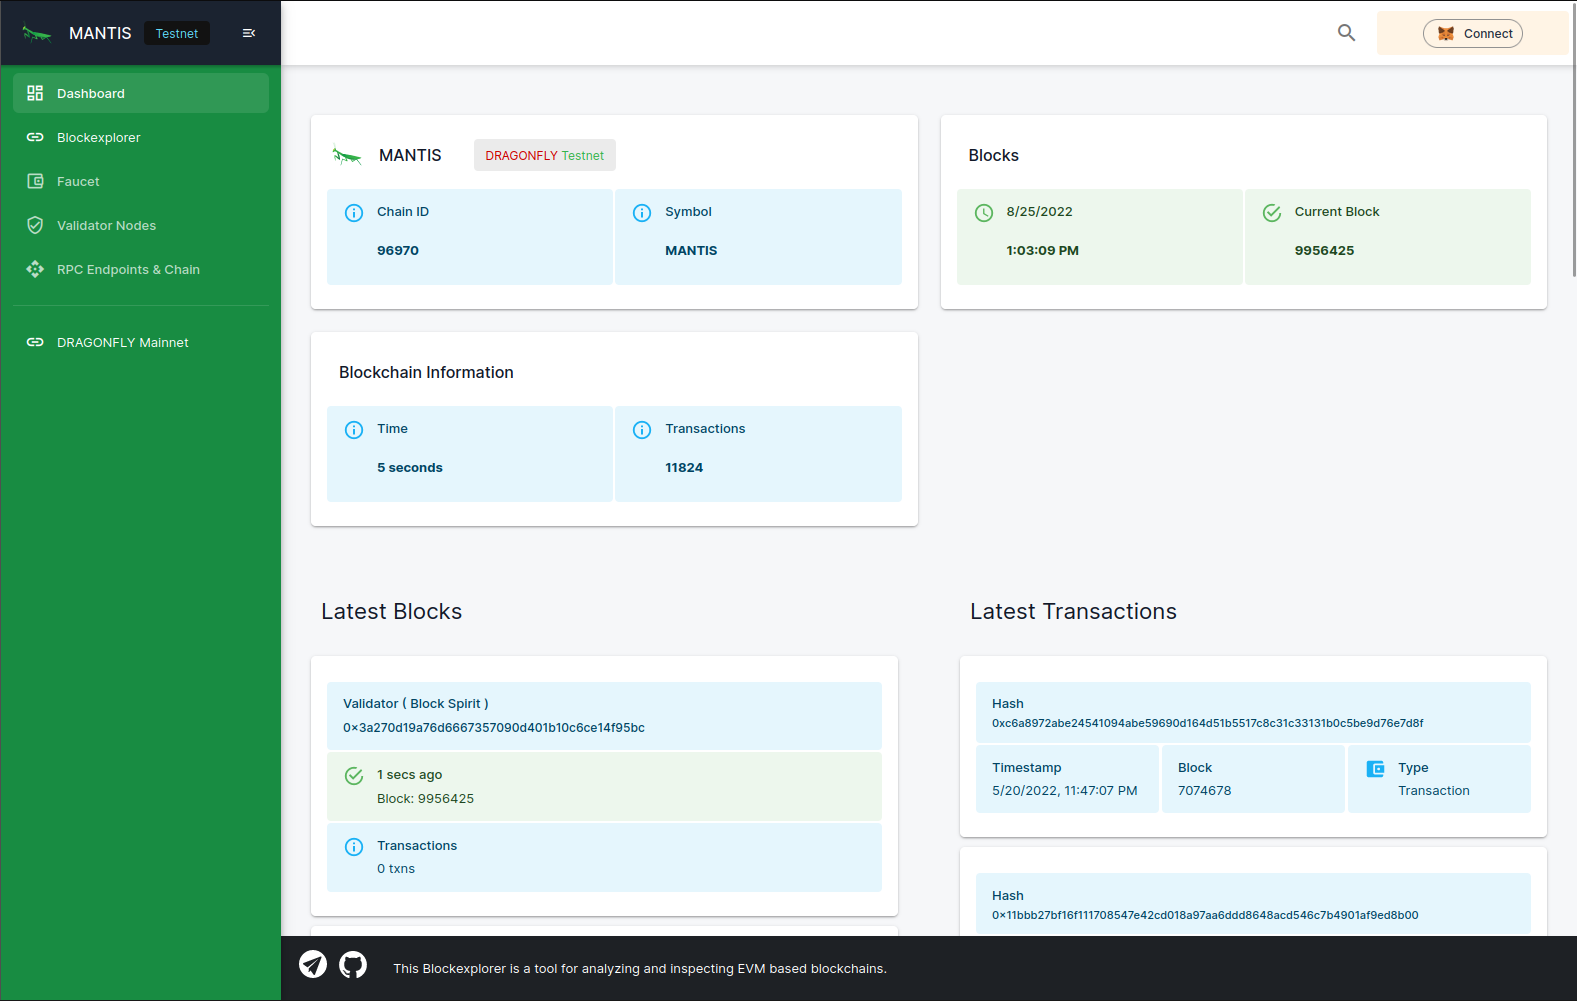
\includegraphics[width=\linewidth]{images/mantis_dashboard.png}%
  \caption{\label{fig:mantis_dashboard}Screenshot of the dashboard of the Mantis testnet.}
\end{figure}

\section{Screenshots}

Below are a few screenshots of the GitDAO demo application.

The homepage is shown in figure \cref{fig:demo_homepage}.
It displays the token that a user owns, the power left in each token as well as the proposal that the user can vote on.

\begin{figure}[ht!]
  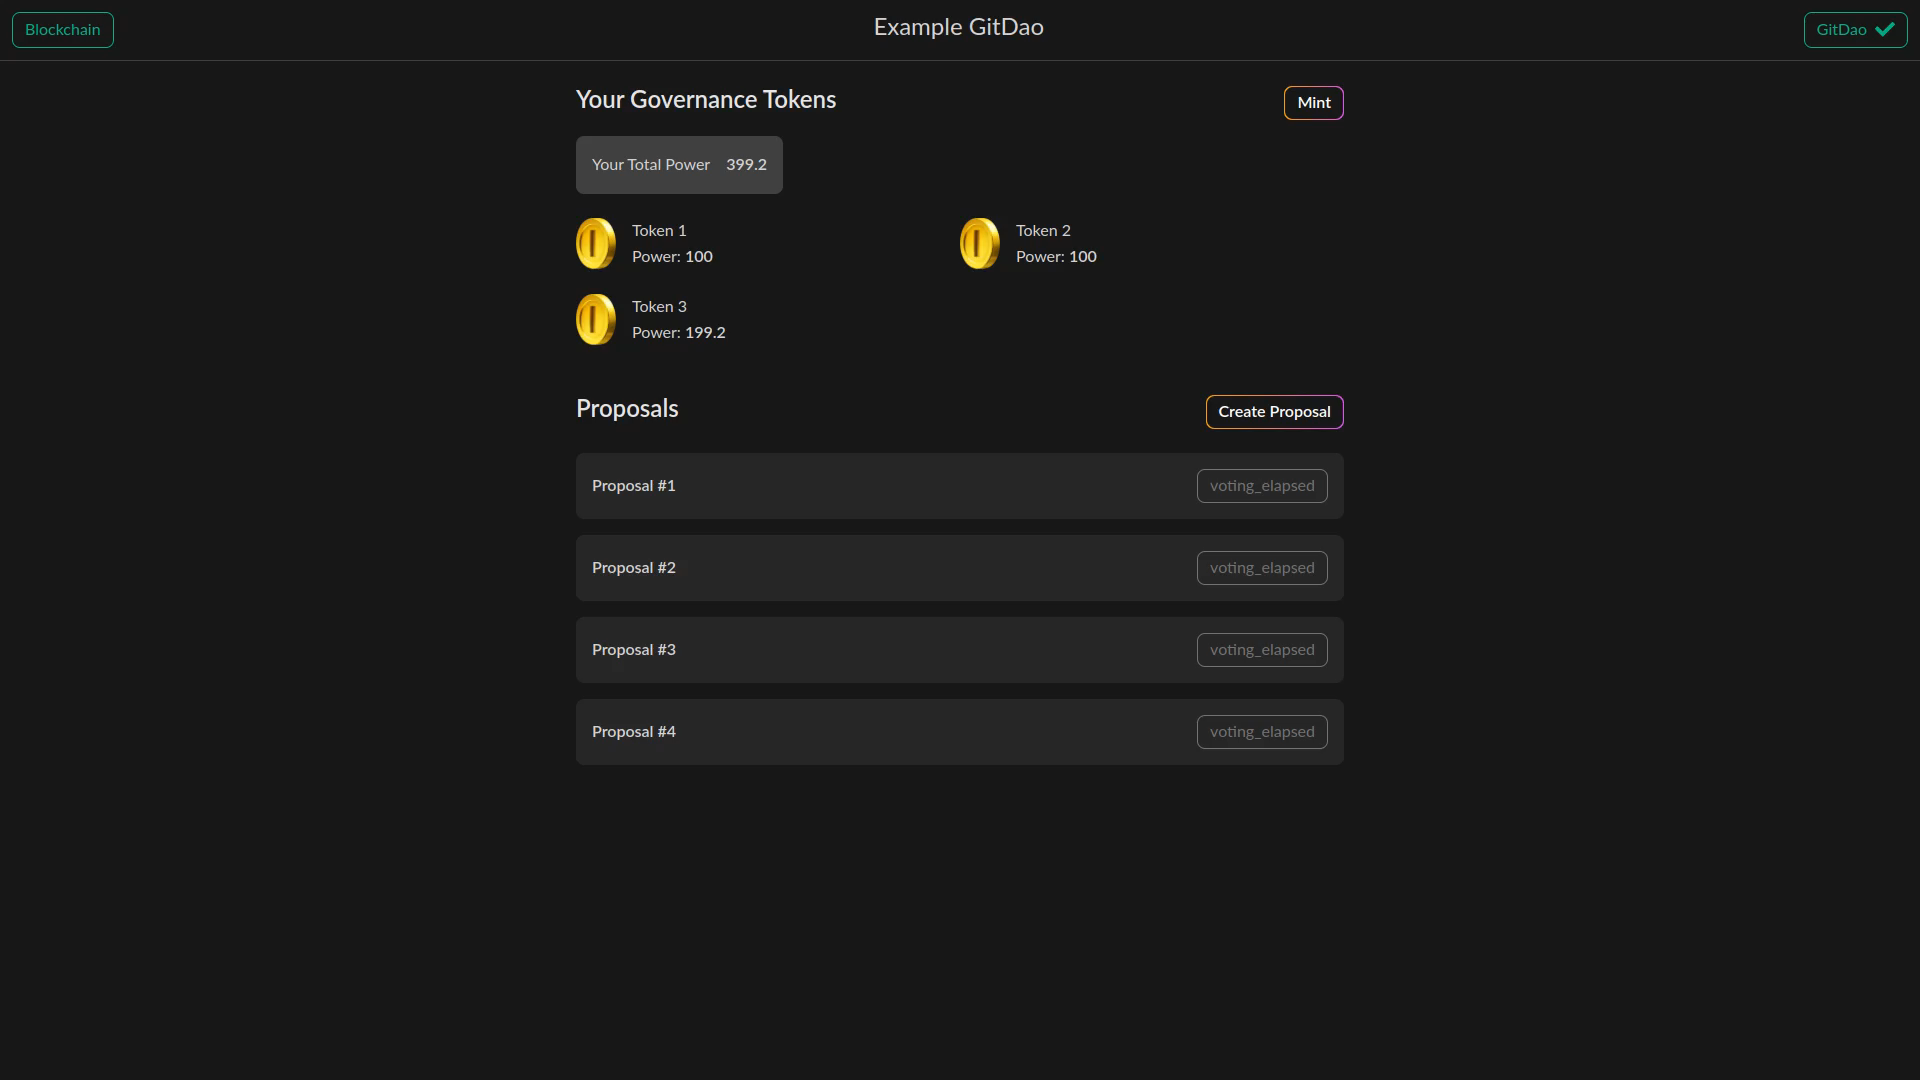
\includegraphics[width=\linewidth]{images/demo/homepage.png}
  \caption{\label{fig:demo_homepage}The homepage of the GitDAO demo.}
\end{figure}

The user can create a proposal, as shown in \cref{fig:demo_proposal_create}.
Once a proposal is created, the user can view it.
At first it will be in the \texttt{Pending} state (see \cref{fig:demo_proposal_read}).
Once the proposal enters the \texttt{Voting Opened} state (shown in \cref{fig:demo_proposal_opened}), the user will be able to vote on the proposal (see \cref{fig:demo_proposal_vote}) and the votes are shown on the proposal page as well (\cref{fig:demo_proposal_voted}).

\begin{figure}[ht!]
  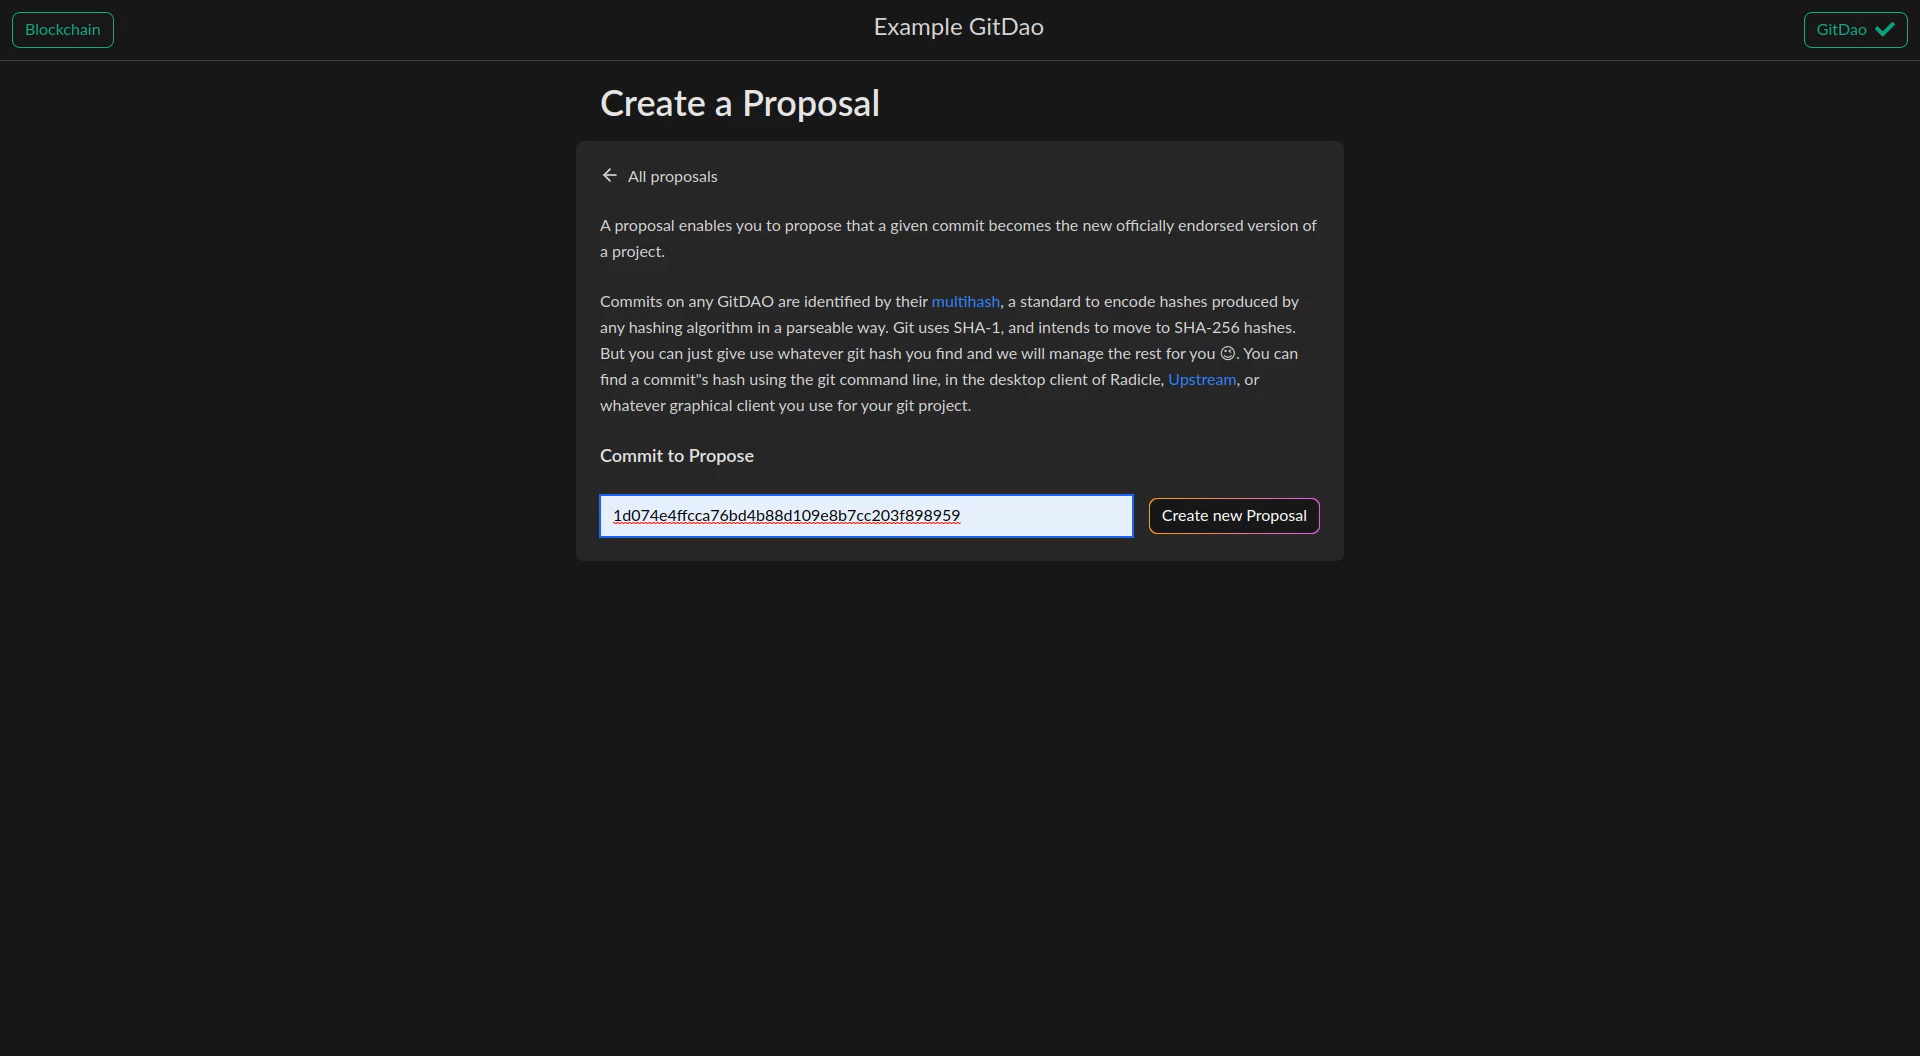
\includegraphics[width=\linewidth]{images/demo/proposal_create.png}
  \caption{\label{fig:demo_proposal_create}The proposal creation screen of the GitDAO demo.}
\end{figure}

\begin{figure}[ht!]
  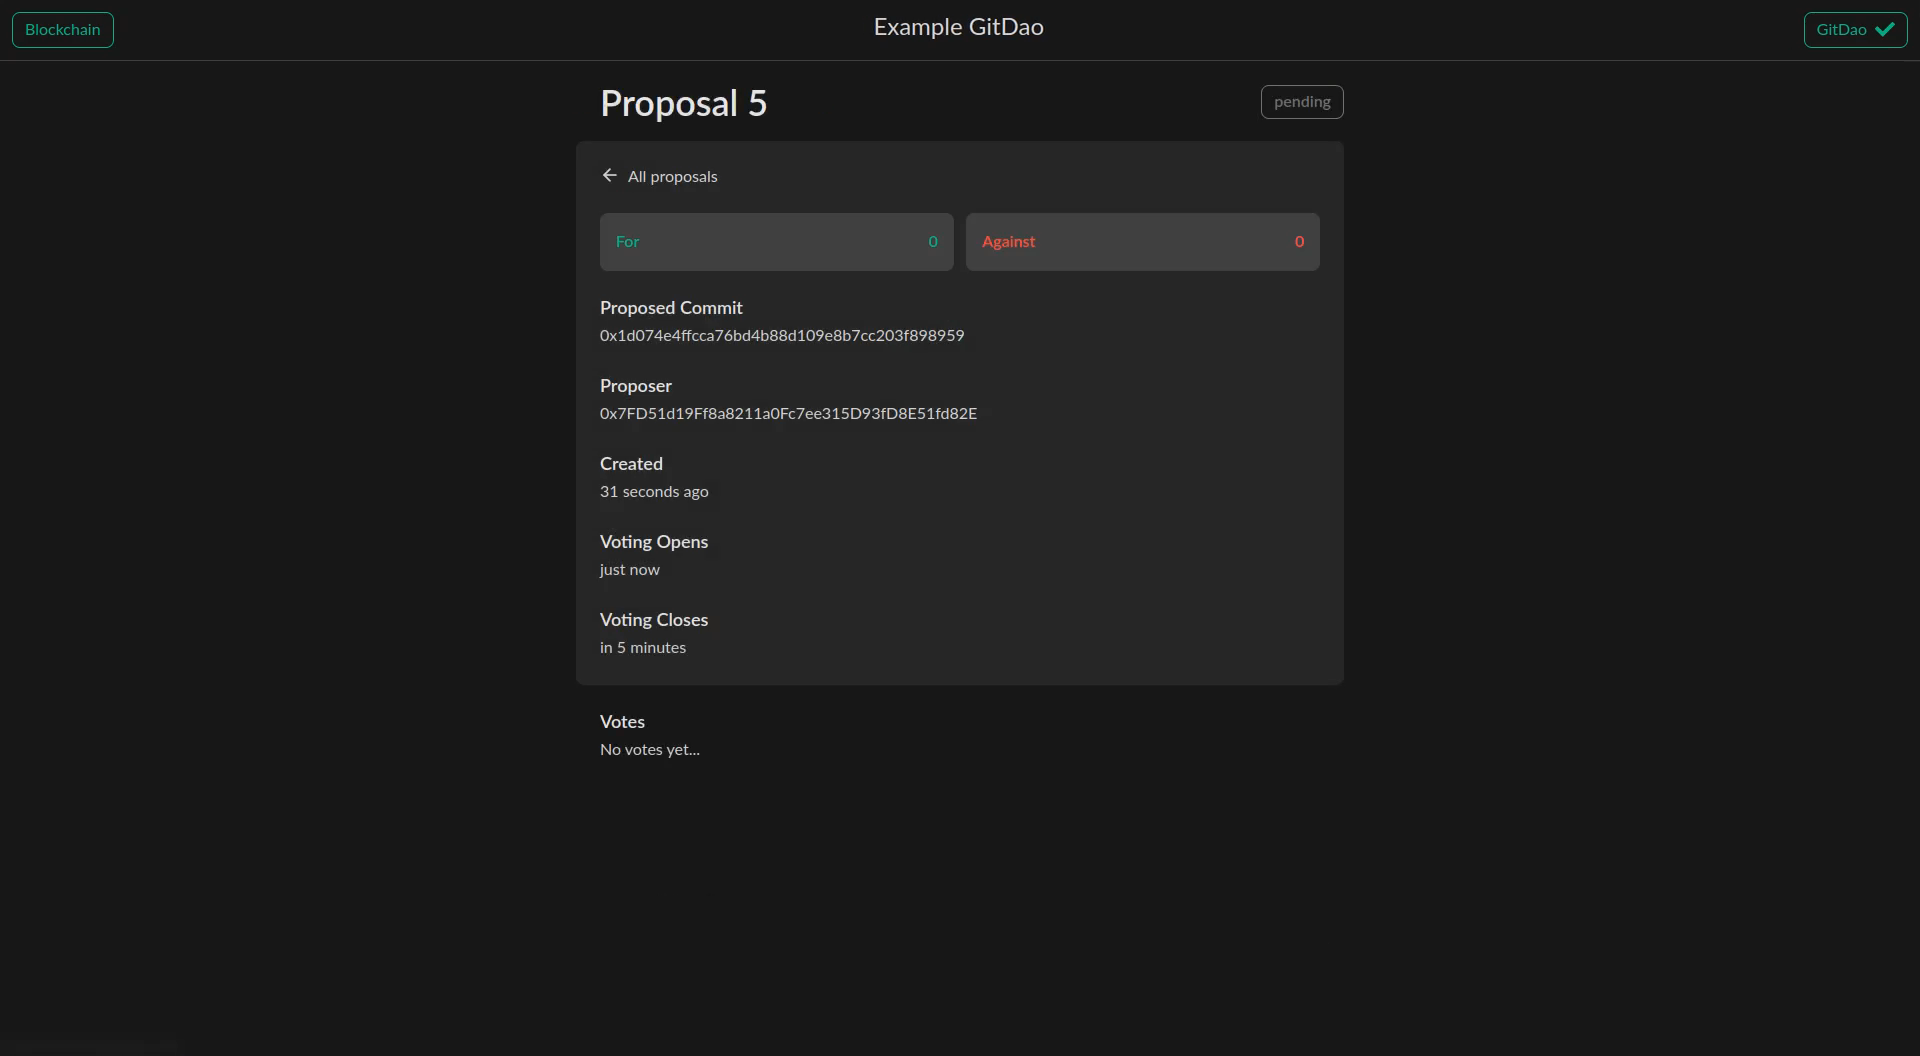
\includegraphics[width=\linewidth]{images/demo/proposal_read.png}
  \caption{\label{fig:demo_proposal_read}A proposal in pending state.}
\end{figure}

\begin{figure}[ht!]
  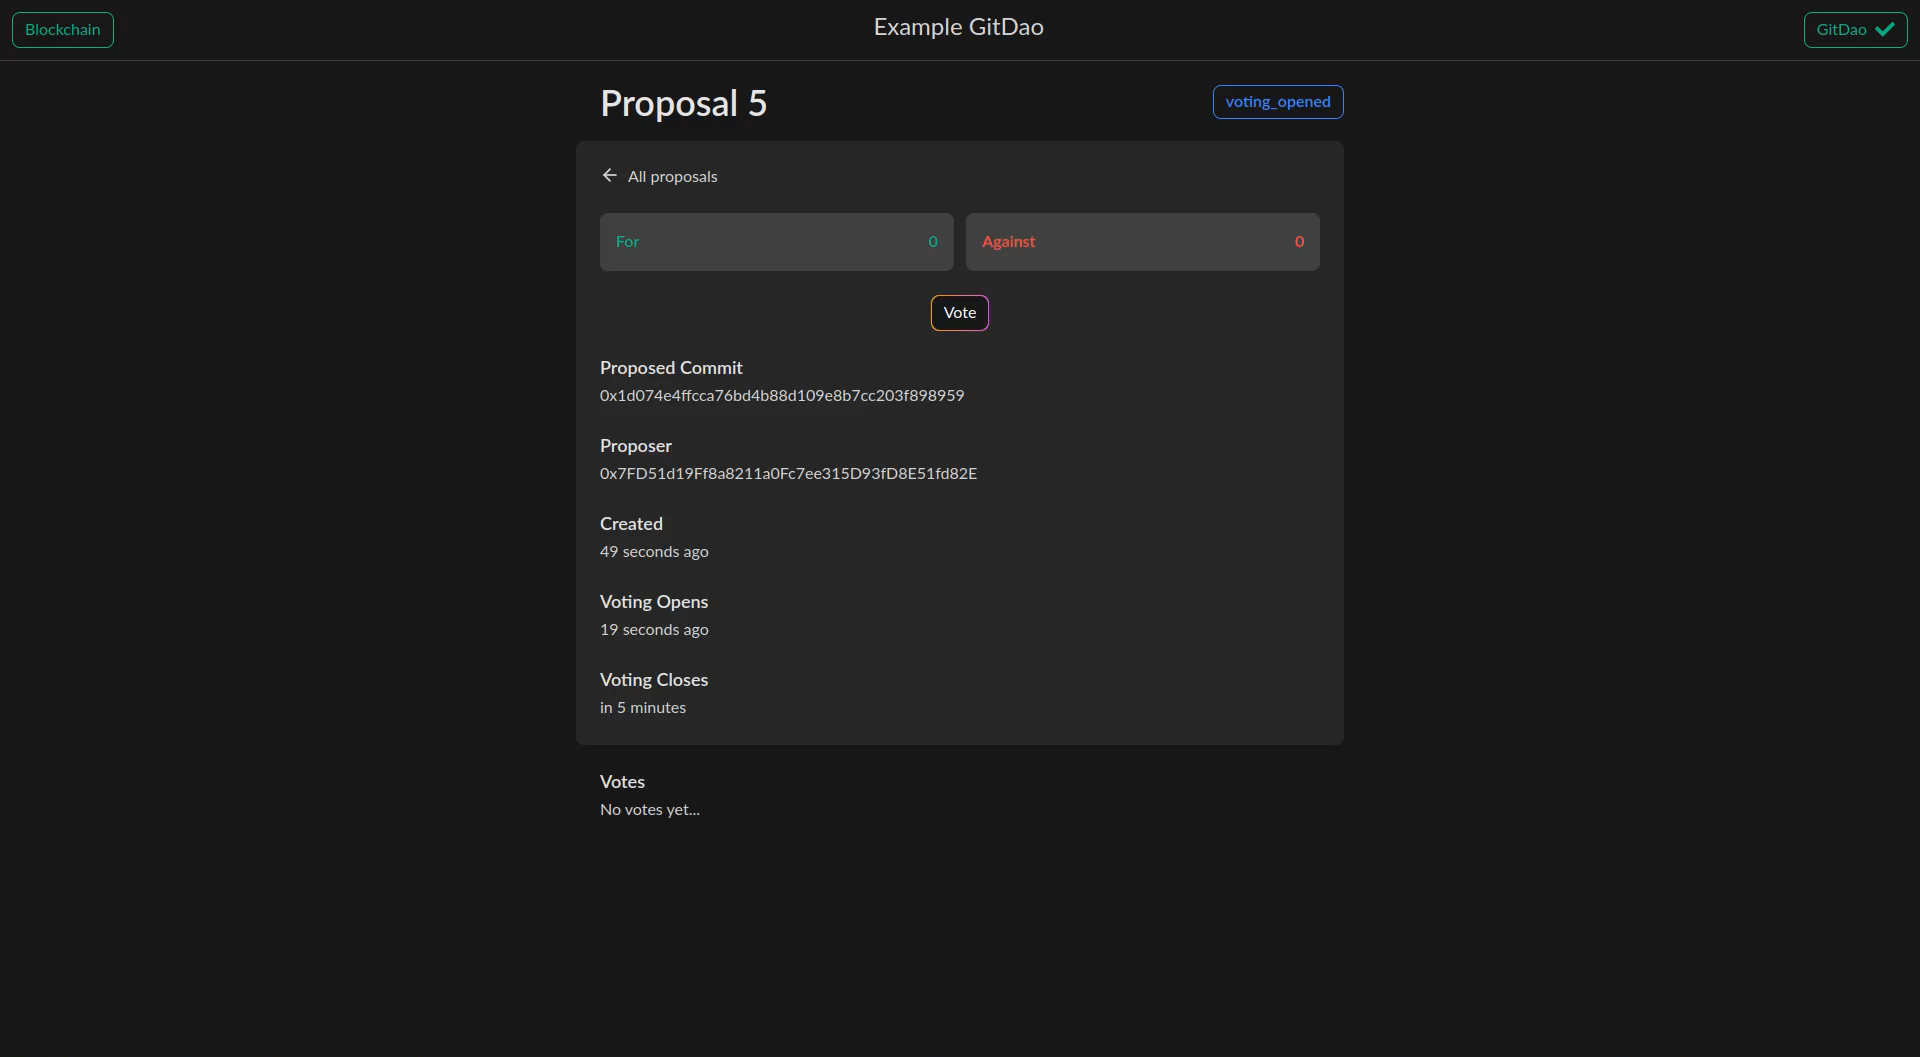
\includegraphics[width=\linewidth]{images/demo/proposal_read_opened.png}
  \caption{\label{fig:demo_proposal_opened}A proposal with voting opened.}
\end{figure}

\begin{figure}[ht!]
  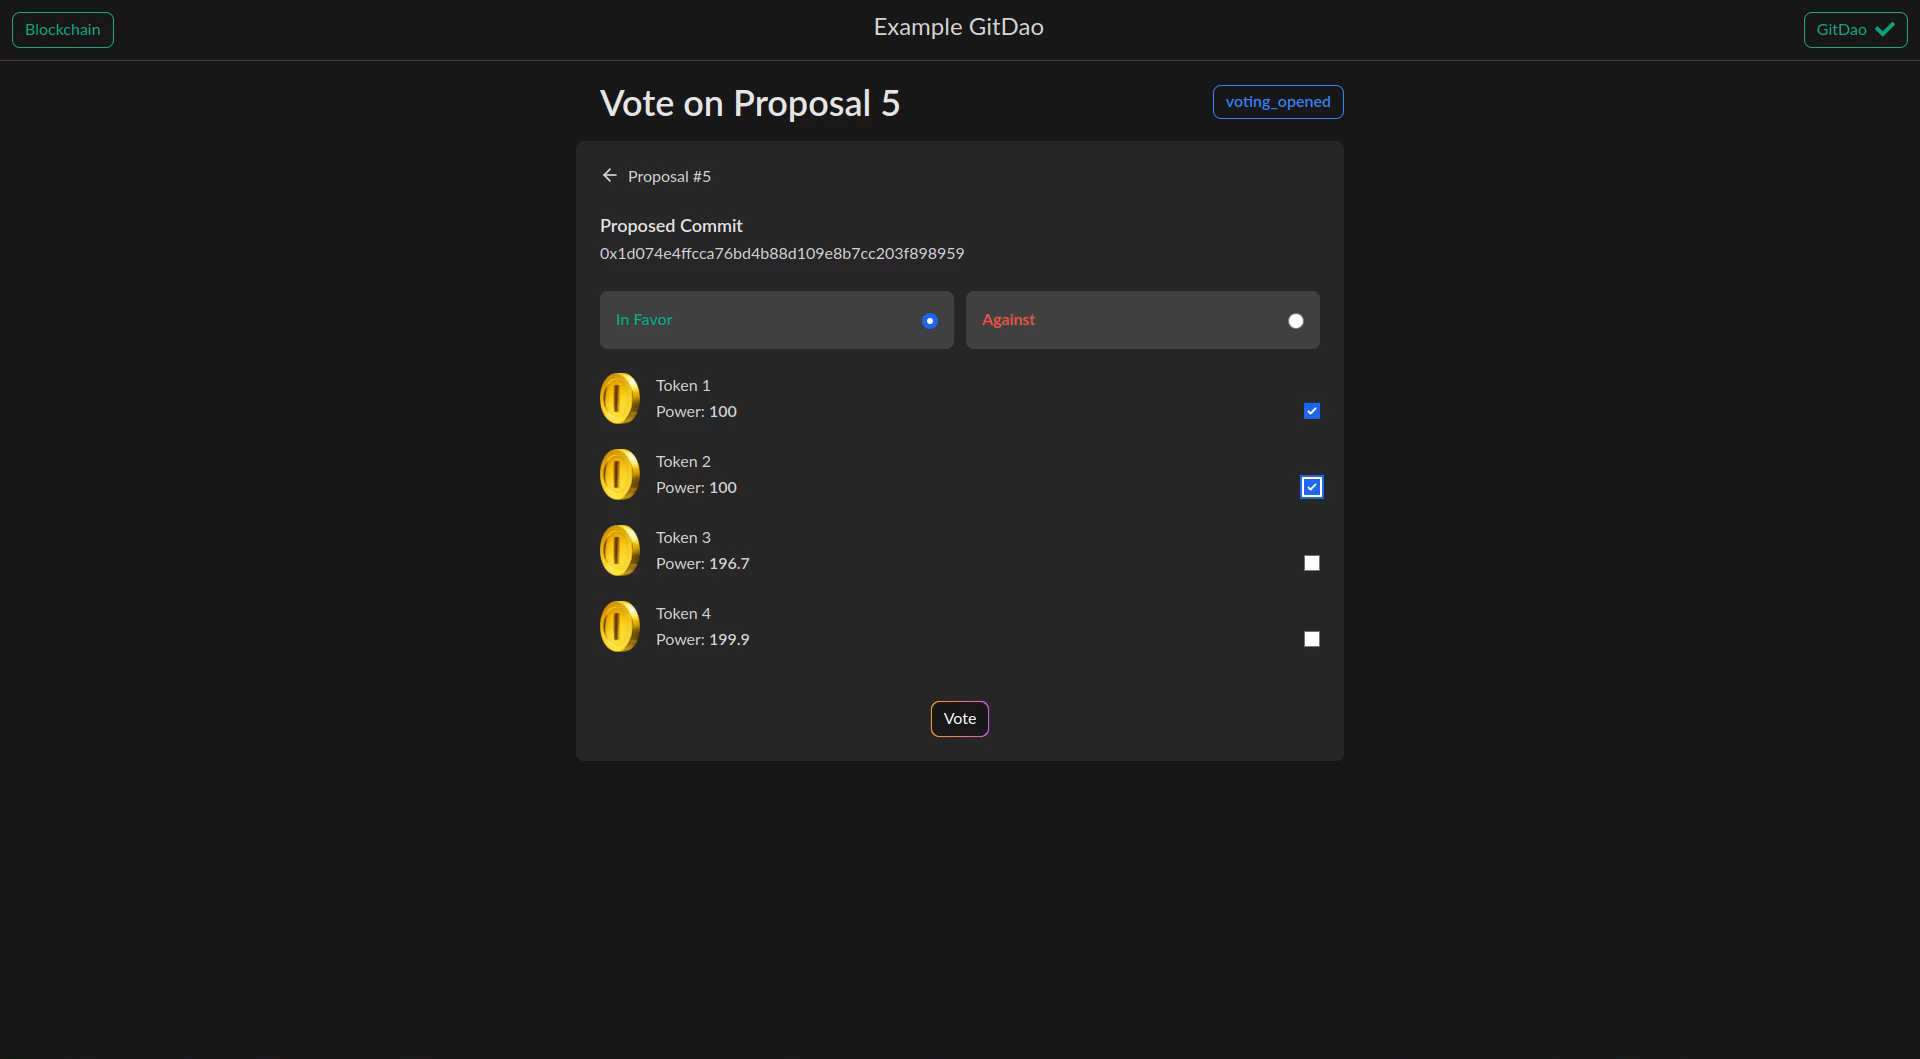
\includegraphics[width=\linewidth]{images/demo/proposal_vote.png}
  \caption{\label{fig:demo_proposal_vote}Voting screen.}
\end{figure}

\begin{figure}[ht!]
  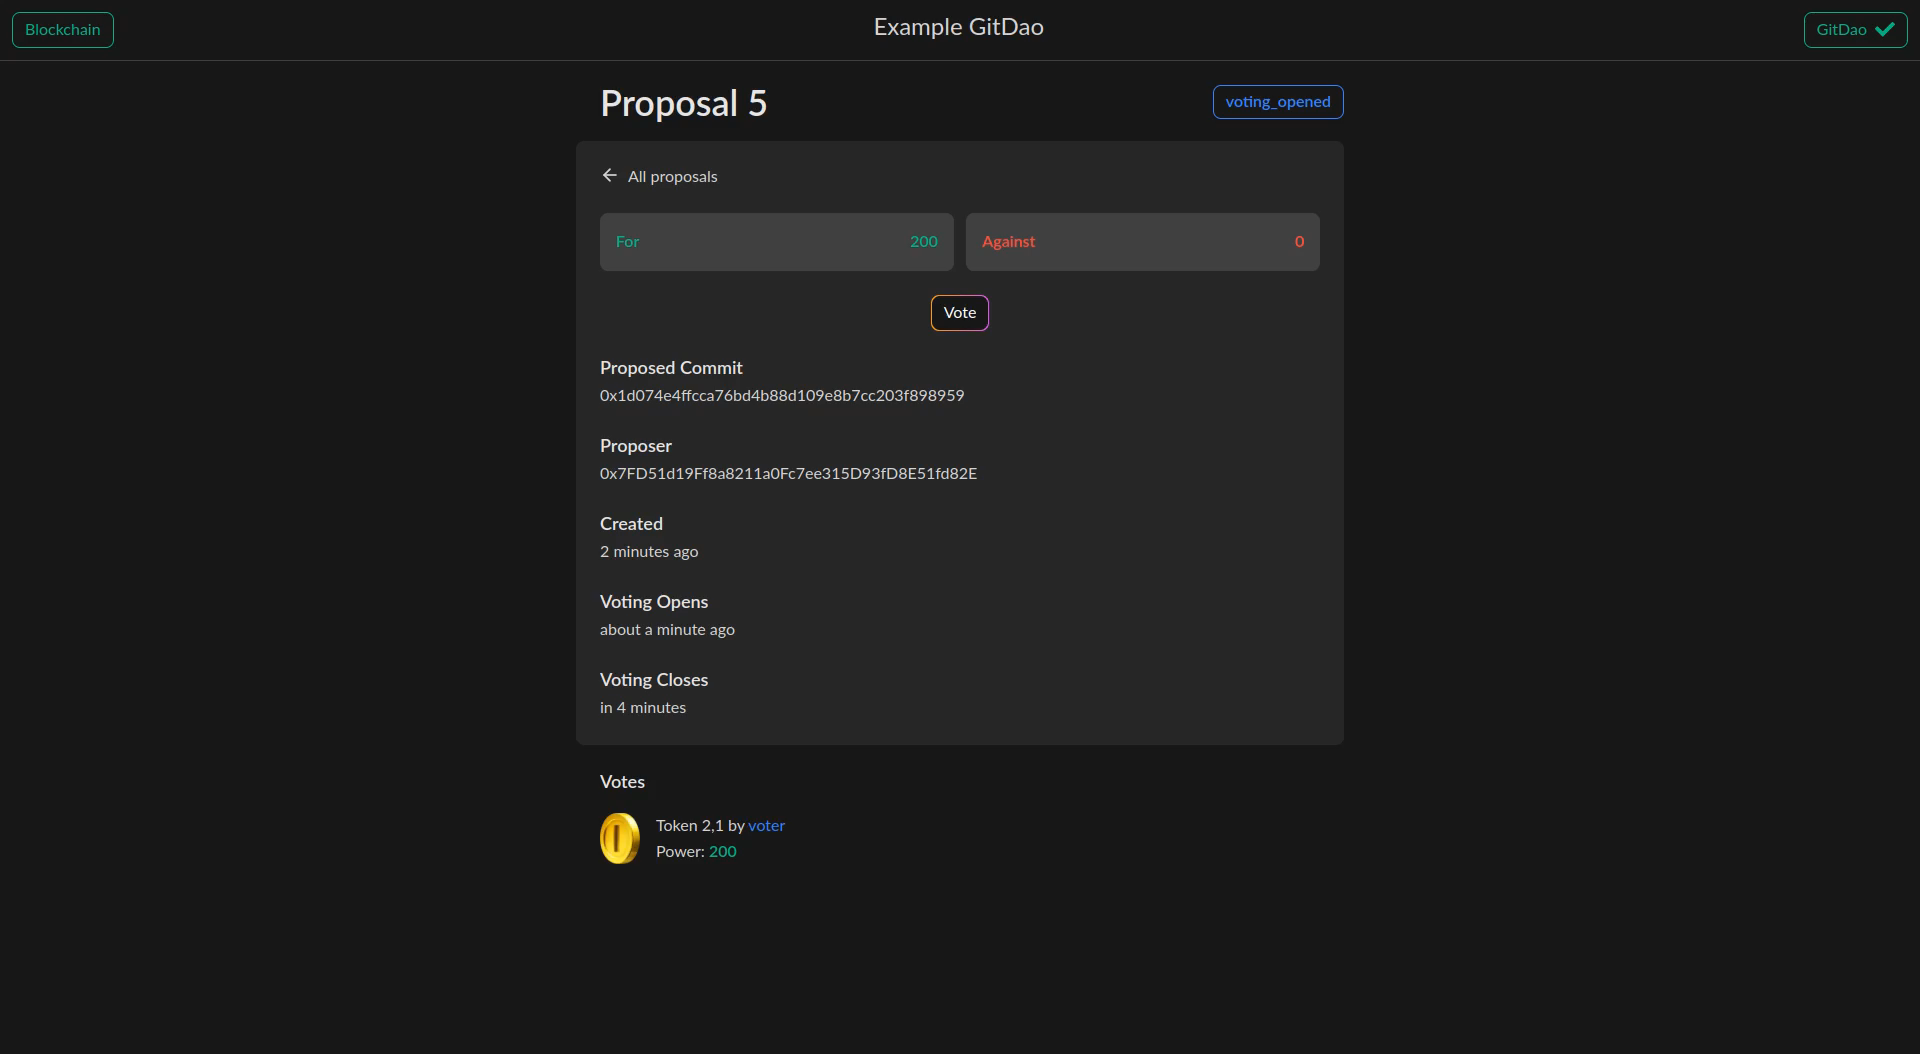
\includegraphics[width=\linewidth]{images/demo/proposal_read_voted.png}
  \caption{\label{fig:demo_proposal_voted}A proposal that received some votes.}
\end{figure}

\section{Development Details}

\marginElement{\centering
\includegraphics[width=.7\linewidth]{images/nix.png}}%
All the git repositories in this project are managed with nix\marginNote{See \href{https://nixos.org/}{nixos.org}.}, a functional package manager.
Nix, besides providing packages, provides a fully reproducible work environment called a nix \enquote{flake} as well as other goodies like command aliases.
This is a powerful tool that provides the guarantee that anyone is able to generate the same outputs in the future.
Through nix flakes it is possible to performs development operations like uploading a website to \textsc{ipfs} and pining this content on Pinata.

The backend code, i.e.\ the GitDAO smart contract is stored in a git repository stored at \url{https://gitlab.com/gitdao/gitdao}.
\marginElement{
  \tikz
    \node[fill=gray_10, inner sep=2mm, text width=\linewidth-4mm]{%
      \includesvg[width=\linewidth]{images/hardhat.svg}
    };
}%
We used hardhat as our Ethereum development environment; it provided us an Ethereum compiler, test frameworks, and tools to deploy to a blockchain of our choosing (like Mantis).

The frontend is a subroute of a blog deployed for this master thesis.
For \textsc{ud}-compatible browsers, use \url{the-git-dao.crypto/app.html}, otherwise the demo is deployed as a Heroku app: \url{https://the-git-dao.herokuapp.com/app}.
The code can be found at \url{https://gitlab.com/gitdao/website}.

